\documentclass[a4paper,11pt]{article}

\usepackage{wrapfig}
\usepackage{amsmath}
\usepackage{pgfplots}
\usepackage{enumerate}
\usepackage{xcolor}
\usepackage[most]{tcolorbox}
%Russian-specific packages
%--------------------------------------
\usepackage[T2A]{fontenc}
\usepackage[utf8]{inputenc}
\usepackage[russian, english]{babel}
%--------------------------------------

\graphicspath{ {./img/} }

\definecolor{lemonchiffon}{rgb}{1.0, 0.98, 0.8}
\newtcolorbox{mainblock}{colback=lemonchiffon,grow to right by=-10mm,grow to left by=-10mm,
boxrule=0pt,boxsep=0pt,breakable} % настройки области с изменённым фоном
\definecolor{block-gray}{gray}{0.95} % уровень прозрачности (1 - максимум)
\newtcolorbox{importantblock}{colback=block-gray,grow to right by=-10mm,grow to left by=-10mm,
boxrule=0pt,boxsep=0pt,breakable} % настройки области с изменённым фоном

\makeatletter
\newcommand{\settag}[1]{
  \tag*{(#1)\qquad}
  \edef\@currentlabel{\theequation#1}}
\makeatother

\title{29. Метод стрельбы для решения краевых задач. Сведение дифференциального уравнения выского порядка
      к системе уравенний первого порядка}
\author{Андрей Бареков \and Ярослав Пылаев \and По лекциям Устинова С.М.}
\date{\today}

\begin{document}
\maketitle
\newpage

\section{Методы решения краевых задач для дифференциальных уравений}
\begin{equation*}
  \frac{dx}{dt} = f(t, x), \hspace{5mm} t \in [a, b].
\end{equation*}
В \textit{задаче Коши} все начальные условия задаются в точке $a$. В общем случае они могут задаваться в любой точке
      на промежутке $[a, b]$, чаще всего их задают на концах (краях) промежутка - такие задачи называются \textit{краевые}. \\

\noindent Методы решения краевых задач делится на две группы, когда исходная задача сводится к
\begin{itemize}
  \item многократному решению зачачи Коши;
  \item решению систем линейных и нелинейных алгебраических уравнений.
\end{itemize}

\noindent Типичным представителем первой группы является \textit{метод стрельбы}.

\subsection{Метод стрельбы (пристрелки)}
Проиллюстрируем на примере уравнения 2-го порядка:
\begin{align*}
  x = \begin{pmatrix} U \\ V \end{pmatrix}, && \frac{dU}{dt} = f_1(t, U, V), && \frac{dV}{dt} = f_2(t, U, V), && t \in [a, b],
\end{align*}
с граничными условиями
\begin{align*}
  \underbrace{U(a) = U_a, V(a) = V_a}, && \underbrace{U(b) = U_b, V(b) = V_b}.
\end{align*}

\noindent Выразим через $U_a$ из левого краевого условия правое условие. Затем методом подбора находим такие значения $U_a^{(1)}$ и $U_a^{(2)}$,
      что $U_b^{(1)} > U_b$, $U_b^{(2)} < U_b$, и реализуем метод бисекции, секущих и т.д. для решения нелинейного уравнения.
\begin{center}
  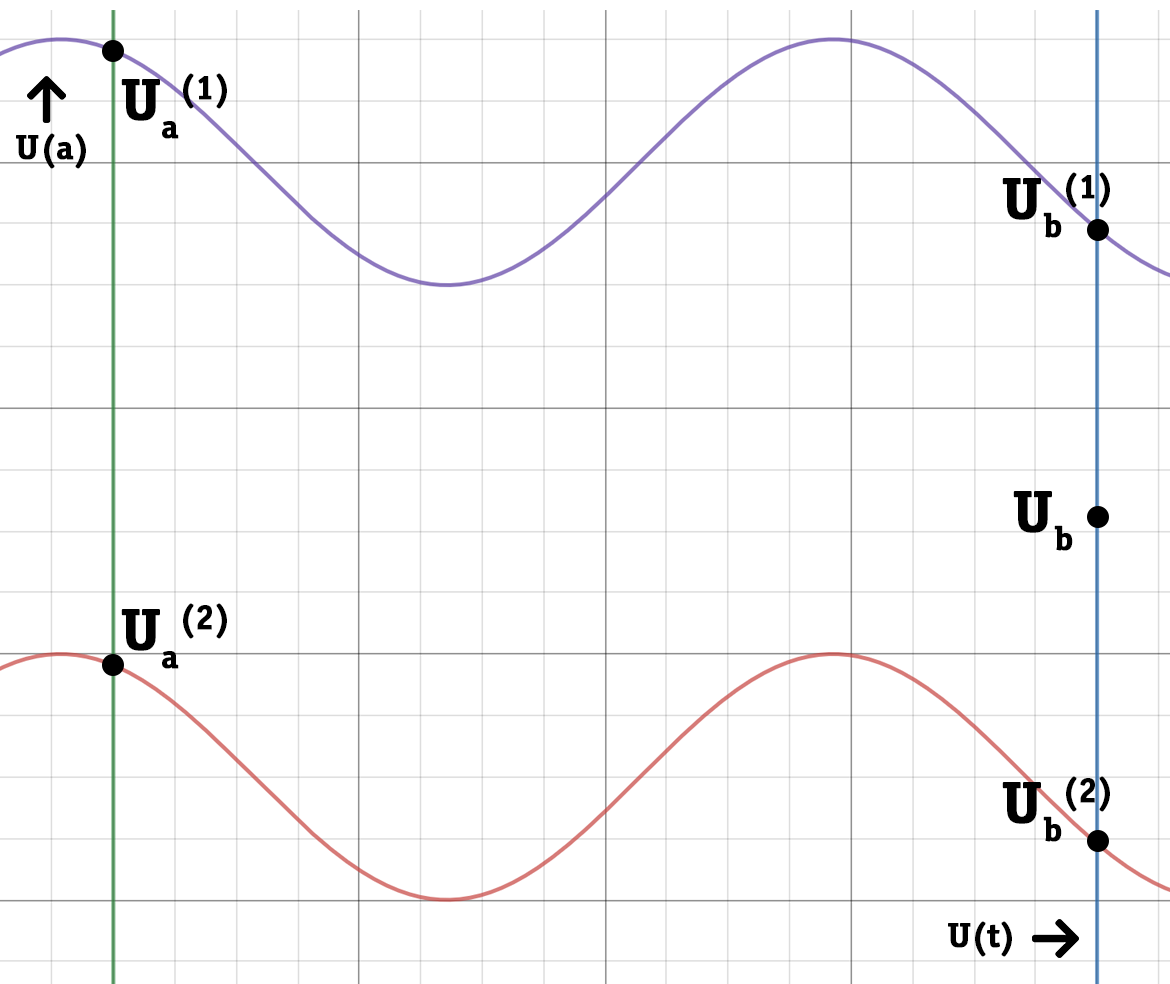
\includegraphics[scale=0.21]{img3.png} \\
\end{center}
\begin{equation*}
  F(U_a) = \underbrace{U(b)}_{compute} - U_b = 0
\end{equation*}
$U(b)$ получается решением системы уравений при помощи \verb|RKF45|, для этих целей еще можно использовать \verb|ZEROIN|.
      Тогда последовательность вызова процедур следующая:

\begin{center}
  \verb|MAIN| \\
  | \\
  \verb|ZEROIN| \\
  | \\
  $F(U_a)$ \\
  | \\
  \verb|RKF45| \\
  | \\
  $f_1(t,U,V), \, f_2(t, U, V)$
\end{center}
\subsubsection{Линейный случай}
\noindent Если исходная система является линейной, то решение линейно зависит от краевых начальных условий
      (функция $F(U_a)$ является линейной). \\

\noindent Строим интерполяционный полином первой степени:
\begin{equation*}
  F(U_a) = \frac{U_a - U_a^{(2)}}{U_a^{(1)} - U_a^{(2)}} F(U_a^{(1)}) + \frac{U_a - U_a^{(1)}}{U_a^{(2)} - U_a^{(1)}} F(U_a^{(2)}) = 0,
\end{equation*}
нужное значение $U_a$ получаем как корень этого полинома.

\section{Сведение дифференциального уравнения высокого порядка к системе дифференциальных уравнений}
\begin{equation*}
  \frac{d^Ny}{dt^N} = F\bigg( t, \frac{d^{N-1}y}{dt^{N-1}}, \frac{d^{N-2}y}{dt^{N-2}}, \cdots, \frac{dy}{dt}, y \bigg)
\end{equation*}
\begin{gather*}
  \text{Выполним замену переменных, введя вектор}
  z = \begin{pmatrix}
    z^{(1)}, \\ z^{(2)}, \\ \dots \\ z^{(N)}
  \end{pmatrix}
\end{gather*}
Компоненты вектора выглядят следующим образом:
\begin{align*}
  & z^{(1)} = \frac{d^{N-1}y}{dt^{N-1}}, \\
  & z^{(2)} = \frac{d^{N-2}y}{dt^{N-2}}, \\
  & \cdots \\
  & z^{(N-1)} = \frac{dy}{dt}, \\
  & z^{(N)} = y.
\end{align*}
Решаем систему ДУ при помощи \verb|RKF45|
\begin{equation*}
  \begin{cases}
    \frac{dz^{(1)}}{dt} = F(t, z^{(1)}, z^{(2)}, \dots, z^{(N)}), \\
    \frac{dz^{(2)}}{dt} = z^{(1)}, \\
    \frac{dz^{(3)}}{dt} = z^{(2)}, \\
    \dots \\
    \frac{dz^{(N)}}{dt} = z^{(N-1)}.
  \end{cases}
\end{equation*}

\end{document}
